\documentclass{beamer}
\usepackage{tikz} 
\usetikzlibrary{calc} 
\usetikzlibrary{matrix}

% Setup appearance:

\usetheme{AnnArbor}
\usecolortheme{beaver}
\usetikzlibrary{arrows,shapes}
\providecommand{\norm}[1]{\lVert #1 \rVert}
\tikzstyle{na} = [baseline=-.5ex]
\tikzstyle{every picture}+=[remember picture] 

\newcommand{\head}[1]{\textnormal{\textbf{#1}}}
\newcommand{\tikzmark}[2]{\tikz[overlay,remember picture,baseline=(#1.base)] \node (#1) {#2};}

\usepackage[font=footnotesize,labelfont=bf]{caption}
\usepackage{amsmath}
\usepackage{xfrac}
\usepackage{multicol}
% Standard packages

\usepackage{algorithm}
\usepackage{algpseudocode}
\usepackage{algorithmicx}
\algdef{SE}[DOWHILE]{Do}{doWhile}{\algorithmicdo}[1]{\algorithmicwhile\ #1}%

%equation
\newcommand{\argmax}[1]{\underset{#1}{\operatorname{arg}\,\operatorname{max}}\;}
\newcommand{\argmin}[1]{\underset{#1}{\operatorname{arg}\,\operatorname{min}}\;}

% Set Front Page
\newcommand\titlegraphicii[1]{\def\inserttitlegraphicii{#1}}
\titlegraphicii{}
\setbeamertemplate{title page}
{
  \vbox{}
  {\usebeamercolor[fg]{titlegraphic}\inserttitlegraphic\hfill\inserttitlegraphicii\par}
 
  \begin{centering}
    \begin{beamercolorbox}[sep=8pt,center]{institute}
      \usebeamerfont{institute}\insertinstitute
    \end{beamercolorbox}
    
    \begin{beamercolorbox}[sep=8pt,center]{title}
      \usebeamerfont{title}\inserttitle\par%
      \ifx\insertsubtitle\@empty%
      \else%
        \vskip0.25em%
        {\usebeamerfont{subtitle}\usebeamercolor[fg]{subtitle}\insertsubtitle\par}%
      \fi%     
    \end{beamercolorbox}%
    
    \vskip1em\par
    \begin{beamercolorbox}[sep=8pt,center]{date}
      \usebeamerfont{date}\insertdate
    \end{beamercolorbox}%\vskip0.5em
    
    % \begin{beamercolorbox}[sep=8pt,center]{author}
    %   \usebeamerfont{author}\insertauthor
    % \end{beamercolorbox}
  \end{centering}
  %\vfill
}

% Front Page
\title{Visual Event Recognition}
\author{Presented by Gong Li}
\date{December 9, 2013}


\begin{document}
\begin{frame}
	\maketitle

\begin{center}
\emph{Supervisor:}
A/P Xu Dong

\vspace{2 mm} 

\emph{Examiner:}
A/P Cham Tat Jen

\vspace{2 mm} 

\emph{Presented by}
Gong Li
\end{center}
\end{frame}


\section{Introduction}
\begin{frame}{Introduction}
\begin{itemize}
	\item Goal - \tikz[baseline]{\node[fill=blue!20,anchor=base] (t1) {recognize various videos};} based on \tikz[baseline]{\node[fill=red!20,anchor=base] (t2) {their content};}
\end{itemize}

\vspace{3mm}

\begin{columns}
	\column{0.5\textwidth}

		\begin{itemize}
			\item Youtube \tikz[na] \node[coordinate] (n1) {}; statistics
				\begin{itemize}
					\item 100 hours of videos are uploaded every minute
					\item Over 6 billion hours of video are watched each month
				\end{itemize}

			\item Vine and Instagram
		\end{itemize}

	
	\column{0.5\textwidth}
		\begin{itemize}
			\item Currently, video \tikz[na] \node[coordinate] (n2) {}; search is heavily relying on texts associated with videos
			\item Explore other approaches to index and retrieve videos
		\end{itemize}
\end{columns}

\begin{tikzpicture}[overlay]
	\draw[line width = 2pt, blue, ->] (t1) -- ($(n1.north)+(0, 0.3)$);
	\draw[line width = 2pt, red, ->] (t2) -- ($(n2.north)+(0, 0.3)$);
\end{tikzpicture}


\end{frame}



\begin{frame}{Outline}
\begin{multicols}{2}
  \tableofcontents
   \end{multicols}
\end{frame}

\AtBeginSection[]
{
  \begin{frame}<beamer>
   \begin{multicols}{2}
     \tableofcontents[currentsection,hideothersection]
   \end{multicols}
  \end{frame}
}


% \include{ImageRec}
\section{Video Recognition}

\subsection{Bag of Words}
\begin{frame}{Naive Bag of Words}

		\begin{tikzpicture}
			\node (video) at (-1, 0) {\includegraphics[scale=0.4]{videoSample.png}};
			\node (videoSIFT) at (2.5,0) {\includegraphics[scale=0.38]{videoSIFT.png}};

			\draw[->, line width = 2pt, black] (video) -- (videoSIFT) node[pos=.5, above] {\scriptsize{Locate}};

			\node (SIFTs) at (6,0) {\includegraphics[scale=0.4]{SIFTs}};
			\draw[->, line width = 2pt, black] (videoSIFT) -- (SIFTs) node[pos=.5, above] {\scriptsize{Describe}};

			\node (his) at (9, 0) {\includegraphics[scale=0.4]{his}};
			\draw[->, line width = 2pt, black] (SIFTs) -- (his) node[pos=.5, above] {\scriptsize{Project}};

		\end{tikzpicture}

		\begin{columns}
			\column{0.48\textwidth}
				\begin{itemize}
					\item $M$: number of sampled frames
					\item $V$: size of visual vocabulary 
				\end{itemize}
			\column{0.6\textwidth}

				\[
					  \left(\begin{array}{*5{c}}
					   	A_{11} & A_{12} & \cdots & \tikz[baseline]{\node[anchor=base] (t1) {$A_{1(V-1)}$};} & A_{1V}\\
						A_{21} & A_{22} & \cdots & A_{2(V-1)} & A_{2V}\\
						\vdots & \vdots & \vdots & \vdots & \vdots\\
						A_{M1} & A_{M2} & \cdots & A_{M(V-1)} & A_{MV}\\
					  \end{array}\right)
			    \]

	    \end{columns}

		\begin{tikzpicture}[overlay]

			\draw[->, line width = 2pt] (his) -- (t1); 

		\end{tikzpicture}
\end{frame}


\begin{frame}{Better Bag of Words - Soft Assignment}
	
	\begin{itemize}
		\item Straightforward approach \cite{jiang2007towards}
			\begin{itemize}
				\item Assign top $N$ nearest words to each feature
				\item Update the histogram by adding different weights to these $N$ words
			\end{itemize}

		\item Gaussian Mixture Models Assignment \cite{agarwal2006hyperfeatures} \\
			\vspace{2mm}
			\begin{tikzpicture}
				\node[draw, fill = gray!30] at (0,0) (trainVideo) {Training Videos};
				\node[draw, fill = gray!30] at (3.1,0) (SIFT) {SIFT Features};

				\node[draw, fill = gray!30] at (7,0) (GMM) {Gaussian Mixture Models};		


				\draw[->, line width = 2pt] (trainVideo) -- (SIFT);
				\draw[->, line width = 2pt] (SIFT) -- (GMM);



				\node (image) at (0,-2) {\includegraphics[scale=0.4]{image.png}};
				\node (oneSIFT) at (2.5,-2) {\includegraphics[scale=0.6]{oneSIFTs.png}};

				\draw[->, line width = 2pt] (image) -- (oneSIFT);

				\node[fill = green!30] (pro1) at (5.5, -1.5) {$[p_1, p_2, \cdots, p_K]$};
				\node[fill = green!30] (pro2) at (5.5, -2) {$[p_1, p_2, \cdots, p_K]$};
				\node (pro3) at (5.5, -2.5) {$\vdots$};
				\node[fill = green!30] (pro4) at (5.5, -3) {$[p_1, p_2, \cdots, p_K]$};

				\draw[->, line width = 2pt] (oneSIFT) -- (pro2) node[pos=.5,above] (middle){};
				\draw[->, line width = 2pt, red] (GMM) edge[bend right] (middle);

				\node (plus) at (7.2, -2.4) {$+$};
				\node[fill = red!30] (pro4) at (8.9, -2.4) {$[P_1, P_2, \cdots, P_K]$};

			\end{tikzpicture}
	\end{itemize}

\end{frame}


\begin{frame}{Better Bag of Words - Weighting Schemes \cite{yang2007evaluating}}
	\begin{itemize}
		\item Inverse document frequency of visual word $t_i$
				\begin{equation}
				idf(t_i) = \log(N / n_i)
				\end{equation}

				\begin{itemize}
					\item $N$ is the total number of images in the corpus
					\item $n_i$ is the number of images having visual word $t_i$
				\end{itemize}

		\item Various different weighting schemes
			
			\begin{table}[!ht]
	        \begin{center}

	        \scalebox{0.7}{
	          \begin{tabular}{ccc}
	          \hline
	          \head{Name} & \head{Factors} & \head{Value for $t_i$}\\
	          \hline
	    		bxx & $binary$ & 1 if $t_i$ presents, 0 if not \\
	    		txx & $tf$ & $tf_i$ \\
	    		txc & $tf, normalization$ & $\frac{tf_i}{\sum_i tf_i}$ \\
	    		tfx & $tf, idf$ & $tf_i \cdot \log(\sfrac{N}{n_i})$ \\
	    		tfc & $tf, idf, normalization$ & $ \frac{tf_i \cdot \log(\sfrac{N}{n_i})}{\sum_i tf_i \cdot \log(\sfrac{N}{n_i})}$ \\
	          \hline
	          \end{tabular}
	         }
	        \end{center}
	        \caption{Weighting schemes for visual-word feature \cite{yang2007evaluating}}
	    	\end{table}

	\end{itemize}
\end{frame}

\begin{frame}{Aligned Space-Time Pyramid Matching \cite{duan2012visual} at level 0}
\begin{itemize}
	\item Incorporate \alert{Earth Mover's Distance} (EMD) \cite{rubner2000earth}

	\item Given two videos $P$ and $Q$
	$$P = \{(p_1, 1 / m),...,(p_m, 1 / m) \}, Q = \{(q_1, 1 / n),...,(q_n, 1 / n) \}$$

	\item Solve the below optimization problem 
	\begin{columns}
		\column{0.6\textwidth}
			\begin{eqnarray}
			\text{minimize} & \sum_{i=1}^{m}\sum_{j=1}^{n}
			\tikz[baseline]{\node[fill=green!40,anchor=base] (t1)
			{$d_{ij}$};}\tikz[baseline]{\node[fill=red!40,anchor=base] (t2) {$f_{ij}$};} \nonumber \\
			\text{subjective to} & f_{ij} \geq 0 \quad \quad 1 \leq i \leq m,  1 \leq j \leq n \nonumber \\
			&\sum_{j=1}^n f_{ij} \leq 1 / m \quad 1 \leq i \leq m \nonumber \\
			&\sum_{i=1}^m f_{ij} \leq 1 / n \quad 1 \leq j \leq n\nonumber \\
			&\sum_{i=1}^{m} \sum_{j=1}^n f_{ij} = 1 
			\end{eqnarray}

		\column{0.4\textwidth}
			\begin{itemize}
				\item \tikz[na] \node[coordinate] (n1) {}; distance between $p_i$ and $q_j$
				\item \tikz[na] \node[coordinate] (n2) {}; flow between $p_i$ and $q_i$
			\end{itemize}

			\begin{figure}[!ht]
				\centering
					\includegraphics[scale=0.25]{./EMD.png}
				\end{figure}
	\end{columns}

	\begin{tikzpicture}[overlay]
		\path[->, green!40, line width = 2pt] (t1) edge [bend left] (n1); 
		\path[->, red!40, line width = 2pt] (t2) edge [bend left] (n2); 
	\end{tikzpicture}

	\item Distance between $P$ and $Q$
	\begin{equation}
	D_{PQ} = \frac{\sum_{i=1}^m \sum_{j=1}^n d_{ij} f_{ij}}{\sum_{i=1}^m\sum_{j=1}^n f_{ij}} 
	\end{equation}

\end{itemize}
\end{frame}


\begin{frame}{Aligned Space-Time Pyramid Matching \cite{duan2012visual} at level $l$}

	\begin{figure}[!ht]
	\centering
		\includegraphics[scale=0.5]{./spaceTime.png}
	\end{figure}

\begin{itemize}
	\item Each video is divided into $8^l$ non-overlapped sub-videos
	\item Given two videos $P$ and $Q$
		$$P = (p_1, \cdots, p_R), Q = (q_1, \cdots, q_R), \text{where } R = 8^l$$
\end{itemize}
\end{frame}

\begin{frame}{Aligned Space-Time Pyramid Matching \cite{duan2012visual} at level $l$}

	\begin{figure}[!ht]
	\centering
		\includegraphics[scale=0.2]{./alignedST.png}
	\end{figure}


		\begin{enumerate}
			\item Calculate pairwise distance matrix $D$
				\begin{itemize}
					\item $D_{ij}$ is the EMD distance between sub-video $p_i$ and $q_i$
				\end{itemize}

			\item Align sub-videos in $P$ with sub-videos in $Q$ 
				\begin{eqnarray}
				& \hat F_{ij} = \argmin{F_{ij}} \sum_{i = 1}^{R} \sum_{j=1}^{R} F_{ij} D_{ij}
				\nonumber \\
				\text{subject to} & \sum_{i=1}^{R} F_{ij} = 1, \quad \forall j \nonumber\\
				&\sum_{j=1}^{R} F_{ij} = 1, \quad \forall i
				\end{eqnarray}

				\begin{equation}
				D_l(P,Q) = \frac{\sum_{i=1}^R \sum_{j=1}^R \hat F_{ij} D_{ij}}{\sum_{i=1}^R \sum_{j=1}^R F_{ij}}
				\end{equation}
		\end{enumerate}


\end{frame}

\begin{frame}{Experiments of Aligned Space-Time Pyramid Matching}
	
	\begin{itemize}
		\item Data set
			\begin{table}[!ht]
			\begin{center}
			\scalebox{0.7}{
			\begin{tabular}{cccccccc}
			\hline
			\head{} & \head{Wedding} & \head{Sports} & \head{Show} & \head{Picnic} & \head{Parade} & \head{Birthday} & \head{Total}\\
			\hline
			Kodak & 27 & 75 & 57 & 6 & 14 & 16 & 195\\   
			\hline
			\end{tabular}
			}
			\end{center}
			\caption{Number of videos in each class from Kodak }
			\end{table}
		\item Kernel types
			\begin{columns}
				\column{0.4\textwidth}
					\begin{table}[!ht]
					    \begin{center}
					      \scalebox{0.75}{
					      \begin{tabular}{cc}
					      \hline
					      \head{Kernel type} & \head{Kernel function}\\
					      \hline
					      Gaussian & $\exp(-\gamma D^2(I_i, I_j)$ \\
					      Laplacian & $\exp(- \sqrt{\gamma} D(I_i, I_j)$ \\
					      ISD & $\frac{1}{\gamma D^2(I_i, I_j) + 1}$ \\
					      ID & $\frac{1}{\sqrt{\gamma}D(I_i, I_j) + 1}$\\
					      \hline
					      \end{tabular}
					      }
					    \end{center}
					\end{table}

				\column{0.6\textwidth}
					\begin{itemize}
						\item $D(I_i, I_j)$ represents the distance between $I_i$ and $I_j$
						\item $\gamma = \frac{1}{A}$, $A$ is the mean value of the squared distances between training samples

						\item \alert{Fused scores}
						\begin{equation}
						f^{Fuse} = \frac{1}{N} \sum_{i=1}^{N} \frac{1}{1 +\exp{(-f_i)}}
						\end{equation} 
					\end{itemize}
			\end{columns}
	\end{itemize}		
\end{frame}

\begin{frame}{Experiments of Aligned Space-Time Pyramid Matching}
	\begin{itemize}
			\item Division of training and testing samples
			\begin{itemize}
				\item randomly select 3 videos from each class as training samples
				\item the rest of videos act as testing samples
			\end{itemize}

			\item Evaluation metric: Mean Average Precision

			\item Experimental results at different levels using histograms built by naive bag of words

				\begin{table}[!ht]
				\begin{center}
				\scalebox{0.7}{
				\begin{tabular} {cccccc}
				\hline
				\head{} & \head{Gaussian} & \head{Laplacian} & \head{ISD} & \head{ID} &\head{Fused scores}\\
				\hline
				Level 0 & $44.38 \pm 2.13$ & $44.90 \pm 2.73$ & $44.01 \pm 2.13$ & $45.36 \pm 3.13$ & $44.33 \pm 2.61$ \\
				Level 1 (Unaligned) &$43.08 \pm 3.14$ &$43.85\pm3.84$ &$43.22\pm3.11$ &$43.85\pm3.56$ &$43.55\pm3.46$ \\
				Level 1 (Aligned)&$43.61\pm2.97$ &$43.40\pm3.18$ &$43.46\pm2.97$ &$43.22\pm3.11$ & $44.08\pm3.25$ \\
				  \hline
				  \end{tabular}
				  }
				\end{center}
				\caption{Means and standard deviations (percent) of MAPs at different levels}
				\end{table}
	\end{itemize}
\end{frame}

\begin{frame}{Experiments of Aligned Space-Time Pyramid Matching}
	\begin{itemize}
		\item Experimental results using histograms built by better bag of words at level $0$ distance
		\begin{table}[!ht]
		\begin{center}
		\scalebox{0.7}{
		\begin{tabular} {cccccc}
		\hline
		\head{} & \head{Gaussian} & \head{Laplacian} & \head{ISD} & \head{ID} &\head{Fused scores}\\
		\hline
		bxx& $40.20 \pm 2.57$ & $38.35 \pm 2.31$ & $39.93 \pm 2.58$ & $38.23 \pm 2.08$ & $39.34 \pm 2.55$ \\
		txx& $44.28 \pm 2.14$ & $44.90 \pm 2.73$ & $44.01 \pm 2.13 $ & $45.36 \pm 3.13 $ & $44.33 \pm 2.61$ \\
		txc& $ 42.15 \pm 4.73$ & $45.01 \pm 3.45$ & $43.47 \pm 4.56$ & $45.38 \pm 3.20$ & $44.11 \pm 3.90$ \\
		tfx& $ 43.76 \pm 2.99$ & $44.14 \pm 3.36$ & $43.61 \pm 3.03$ & $44.05 \pm 3.51$ & $44.18 \pm 3.22$ \\

		\alert{tfc}& $ 43.71\pm 1.37$ & $\mathbf{46.02 \pm 1.84}$ & $\mathbf{44.93 \pm 1.64}$ & $\alert{\mathbf{46.21 \pm 1.83}}$ & $\mathbf{45.28 \pm 1.62}$ \\
		Easy soft& $43.54 \pm 2.12$ & $ 44.77\pm 2.41$ & $43.52 \pm 2.08$ & $45.24 \pm 2.47$ & $ 44.79\pm 2.55$ \\
		\alert{Gaussian soft}& $\mathbf{44.77 \pm 2.80}$ & $45.23 \pm 2.76$ & $44.90 \pm 3.01$ & $45.23 \pm 2.87$ & $\mathbf{45.20 \pm 3.04}$ \\
		\hline
		\end{tabular}
		}
		\end{center}
		\caption{Means and standard deviations (percent) of MAPs using different mechanisms to build histograms at level 0}
		\end{table}
	\end{itemize}
\end{frame}


\subsection{Gaussian Mixture Models}
\begin{frame}{Gaussian Mixture Models to Represent Videos \cite{zhou2008sift}}

\begin{columns}
	\column{0.5\textwidth}
			\begin{figure}[!ht]
				\centering
					\includegraphics[scale=0.2]{./gmm.png}
				\end{figure}		

	\column{0.6\textwidth}
		\begin{itemize}
			\item Global GMM built from training data
			\item Specialized GMM by adaption
		\end{itemize}
\end{columns}

\begin{itemize}
	\item Specialized GMM of video $P$ and $Q$
		$$P = (\mu_1^p, \cdots, \mu_K^p), Q = (\mu_1^q, \cdots, \mu_K^q)$$
	\item Given global GMM as $\Theta = \{w_1, \mu_1, \Sigma_1, \cdots\}$, the distance of $P$ and $Q$
	\begin{equation}
	d(P,Q) = \frac{1}{2} \sum_{k= 1}^{K} w_k (\mu_k^p - \mu_k^q)^T \Sigma_k^{-1} (\mu_k^p - \mu_k^q)
	\end{equation}
\end{itemize}

\end{frame}

\begin{frame}{Experiments on GMM}

\begin{table}[!ht]
  \begin{center}
  \scalebox{0.7}{
    \begin{tabular} {cccccc}
    \hline
    \head{} & \head{Gaussian} & \head{Laplacian} & \head{ISD} & \head{ID} &\head{Fused scores}\\
    \hline
    spherical 128& $24.70 \pm 1.41 $ & $ 43.04 \pm 1.61 $ & $26.92 \pm 1.00$ & $\alert{\mathbf{43.64 \pm 0.96}}$ & $ 32.91 \pm 2.20$ \\
    spherical 64& $ 23.99 \pm 1.40$ & $42.35 \pm 1.64$ & $ 25.62\pm 1.11$ & $43.42 \pm 1.18$ & $29.01 \pm 1.10$ \\
    full 128& $ 25.69 \pm 7.57 $ & $21.39 \pm 7.32$ & $26.49 \pm 8.38$ & $21.93 \pm 7.75$ & $21.79 \pm 7.29$ \\
    full 64& $  25.23 \pm 0.94$ & $ 29.69 \pm 1.81$ & $25.68 \pm 1.34$ & $30.74 \pm 1.67$ & $26.74 \pm 1.63$ \\
    \hline
    \end{tabular}
    }
    \end{center}
    \caption{Means and standard deviations (percent) of MAPs using different GMMs}
\end{table}

\begin{itemize}
	\item Spherical covariance using ID kernel performed the best
	\item Spherical covariance performed better than full covariance
\end{itemize}
\end{frame}

\subsection{Concept Attributes}
\begin{frame}{Concept Attributes to Represent Videos \cite{liu2013video}}
		\begin{tikzpicture}
			
			\node[draw, fill = gray!30] (trainVideos) at (2, 2.7) {Training Videos};

			\node[fill = green!20] (clf1) at (4,1) {classifier $1$};
			\node[fill = green!20] (clf2) at (4,0.2) {classifier $2$};
			\node[] (clf3) at (4,-0.5) {$\vdots$};
			\node[fill = green!20] (clf4) at (4,-1.3) {classifier $n$};

			\draw[black,thick,dotted] ($(clf1.north west)+(-0.2,0.3)$)  rectangle ($(clf4.south east)+(0.2,-0.3)$);

			\draw[->, line width = 2pt] (trainVideos) -- ($(clf1.north)+(0,0.3)$) node[pos= 0.6, above] {\scriptsize{Train}};

			\node (video) at (0, 0) {\includegraphics[scale=0.4]{videoSample.png}};
			\draw[->, line width = 2pt] (video) -- ($(clf2.west)+(-0.3, -0.2)$) node[pos=.5, above] {Input};

			\node[fill = red!20] (ca) at (7, 0) {$[c_1, c_2, \cdots, c_n]$};
			\draw[->, line width = 2pt] ($(clf2.east)+(0.2, -0.2)$) -- (ca);

			\node(c) at (7, -1) {\small{Concept Attributes}};


			\node[draw, fill = gray!30] (svm) at (10, 0) {SVM};
			\draw[->, line width = 2pt] (ca) -- (svm) node[pos=0.5, above] {\scriptsize{Classify}};
		\end{tikzpicture}

			\begin{enumerate}
				\item Recognize complex events
				\item Make use of pre-trained detectors (even by others)
			\end{enumerate}

\end{frame}

\begin{frame}{Experiments on Concept Attributes}

	  \begin{table}[!ht]
    \begin{center}
    \scalebox{0.7}{
      \begin{tabular}{cccccccc}
      \hline
      \head{} & \head{Wedding} & \head{Sports} & \head{Show} & \head{Picnic} & \head{Parade} & \head{Birthday} & \head{Total}\\
      \hline
      Kodak & 27 & 75 & 57 & 6 & 14 & 16 & 195\\
      Youtube & 91 & 260 & 200 & 85 & 119 & 151 & 906\\
      \hline
      \end{tabular}
    }
    \end{center}
    \caption{Number of videos in each class from Kodak and Youtube}
  \end{table}

	\begin{table}[!ht]
	  \begin{center}
    \scalebox{0.7}{
	    \begin{tabular} {cc}
	    \hline
	    \head{} & \head{Recognition Accuracy}\\
	    \hline
	    Kodak $\to$ Kodak & $38.5 \pm 12.7$\\
	    Youtube $\to$ Kodak & $30.0 \pm 6.9$\\
	    Baseline & $41.6 \pm 11.5$\\
	    \hline
	    \end{tabular}
		}
	    \end{center}
	    \caption{Means and standard deviations (percent) of recognition accuracies}
	\end{table}

\end{frame}

\subsection{Compressed Videos}
\begin{frame}{Compress Videos}

	\begin{enumerate}
		\item Run K-Means on sampled frames of a video
		\item Build a graph for each cluster
		\item Choose representative frames from each graph
	\end{enumerate}

			\begin{figure}[!ht]
				\centering
				\includegraphics[scale=0.32]{./keyFrames.png}
			\end{figure}
\end{frame}

\begin{frame}{Experiments on Compressed Videos}

\begin{itemize}
	\item Size of Youtube videos is compressed from 4.42 GB to 3.17 GB. ($28.41 \%$ reduced)
	
	\vspace{5mm}
	\begin{table}[!ht]
  	\begin{center}
  	\scalebox{0.7}{
    \begin{tabular} {cccc}
    \hline
    \head{Training videos} & \head{Testing videos} &\head{Original videos} &\head{Compressed videos}\\
    \hline
    60 & 846 &  $38.9 \pm 2.9$  & $38.6 \pm 2.8$ \\
    120 & 786 & $45.7 \pm 2.2$  & $44.5 \pm 1.6$ \\
    180 & 726 & $49.5 \pm 1.8$  & $48.3 \pm 1.9$ \\
    240 & 666 & $52.0 \pm 2.1$  & $50.6 \pm 2.1$\\
    \hline
    \end{tabular}
    }
    \end{center}
    \caption{Means and standard deviations (percent) of MAPs over six events}
	\end{table}
\end{itemize}
		
	\begin{enumerate}	
		\item Compressed videos performed slightly worse than original videos
		\item With more training samples, the performance increases
	\end{enumerate}

\end{frame}
\section{Domain Adaptations}
\begin{frame}{Domain Adaptations}
	
			\begin{figure}[!ht]
				\centering
				\includegraphics[scale=0.15]{./domainAdaption.png}
			\end{figure}


			\begin{itemize}
				\item Feature Replication \cite{daume2007frustratingly} (FR)
				\item Adaptive Support Vector Machine \cite{yang2007cross} (A-SVM)
				\item Domain Transfer Support Vector Machine \cite{duan2009domain} (DTSVM)
				\item Adaptive Multiple Kernel Learning \cite{duan2012visual} (A-MKL)
			\end{itemize}

\end{frame}






\subsection{Feature Replication}
\begin{frame}{Feature Replication (FR)}
	\begin{itemize}
		\item Mapping functions to augment samples $\{x\}$ from different domains

\begin{equation}\Phi^T(\mathbf{x}) = (\mathbf{x},\mathbf{x},\mathbf{0}), \quad  \Phi^A(\mathbf{x}) = (\mathbf{x},\mathbf{0}, \mathbf{x})\end{equation}

		\item \alert{Kernelized} meaning of the above augmenting\\

			\begin{itemize}
			\item If $x_i$ and $x_j$ come from the same domain, 
\begin{eqnarray}
\hat K(x_i, x_j) &  = & \theta(x_i)^T \cdot \theta(x_j) + \theta(x_i)^T \cdot \theta(x_j) \nonumber \\
 & = & 2 K(x_i, x_j)
\end{eqnarray}

			\item If  $x_i$ and $x_j$ come from different domains,
\begin{eqnarray}
\hat K(x_i, x_j)  & = &  \theta(x_i)^T \cdot \theta(x_j)  \nonumber \\
 & = &  K(x_i, x_j) 
\end{eqnarray}
			\end{itemize}

		\item To summarize,
\[
 \hat K(x_i, x_j) =
  \begin{cases}
   2 K(x_i, x_j) & \text{if } x_i \text{ and } x_j \text{ come from the same domain}\\
   K(x_i, x_j)   & \text{otherwise} 
  \end{cases}
\]		
	\end{itemize}
\end{frame}

\subsection{Adaptive SVM}
\begin{frame}{Adaptive Support Vector Machine (A-SVM)}


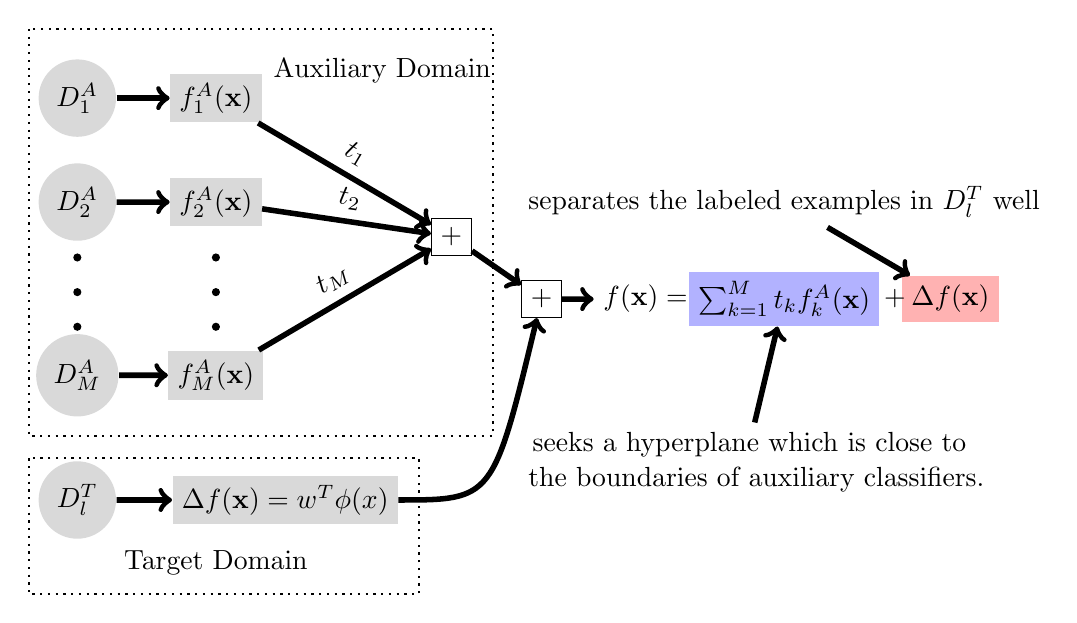
\begin{tikzpicture} [scale = 0.88] 
% Auxiliary Domain
\node[circle, fill = gray!30] (one) at (0, 0) {$D^A_1$};
\node[circle, fill = gray!30] (two) at +(-90: 1.5) {$D^A_2$};

\draw[fill=black] +(-90:2.3) circle (0.05);
\draw[fill=black] +(-90:2.8) circle (0.05);
\draw[fill=black] +(-90:3.3) circle (0.05);

\node[circle, fill = gray!30] (three) at +(-90: 4) {$D^A_M$};


\node[rectangle, fill = gray!30] (cone) at (0: 2) {$f_1^A(\mathbf{x})$};
\node[rectangle, fill = gray!30] (ctwo) at (2, -1.5) {$f_2^A(\mathbf{x})$};

\draw[fill=black] +(2, -2.3) circle (0.05);
\draw[fill=black] +(2, -2.8) circle (0.05);
\draw[fill=black] +(2, -3.3) circle (0.05);

\node[rectangle, fill = gray!30] (cthree) at (2,-4) {$f_M^A(\mathbf{x})$};


\node[draw] (plus) at (5.4, -2) {$+$};

% Add edges
\draw[->, line width = 2pt] (one) -- (cone);
\draw[->, line width = 2pt] (two) -- (ctwo);
\draw[->, line width = 2pt] (three) -- (cthree);

\draw[->, line width = 2pt] (cone) -- (plus) node[pos= 0.5, sloped, above]{$t_1$};
\draw[->, line width = 2pt] (ctwo) -- (plus) node[pos= 0.5, sloped, above]{$t_2$};
\draw[->, line width = 2pt] (cthree) -- (plus) node[pos= 0.5, sloped, above]{$t_M$};

\draw[black,thick,dotted] ($(one.north west)+(-0.3,0.6)$)  rectangle ($(plus.south east)+(0.3,-2.6)$);

\node (auxiliary) at ( 4.4, 0.4) {Auxiliary Domain};

% Target Domain
\node[circle, fill = gray!30] (t) at (0, -5.8) {$D^T_l$};
\node[rectangle, fill = gray!30] (tF) at (3, -5.8) {$\Delta f(\mathbf{x}) = w^T \phi(x)$};
\node[draw](plus2) at (6.7,-2.9) {$+$};

\draw[->, line width = 2pt] (t) -- (tF);
\draw[->, line width = 2pt] (plus) -- (plus2);
\draw[->, line width = 2pt] (tF) .. controls +(right: 3) .. (plus2);

\draw[black,thick,dotted] ($(t.north west)+(-0.3,0.2)$) rectangle ($(tF.south east)+(0.3,-1)$);

\node (target) at (2, -6.7) {Target Domain};

% Decision Function
\node[rectangle] (df) at (8.2, -2.9) {$f(\mathbf{x})=$};

\node[fill = blue!30](partOne) at (10.2, -2.9) {$\sum_{k=1}^M t_k f_{k}^A(\mathbf{x})$};
\node[fill= red!30](partTwo) at (12.6, -2.9) {$ \Delta f(\mathbf{x})$};
\node at (11.8, -2.9) {$+$};

\draw[->, line width = 2pt] (plus2) -- (df);


% Two key points of decision function
\node (keyOne) at (10.2, -1.5) {separates the labeled examples in $D^T_l$ well};

\node (keyTwo) at (9.7, -5) {seeks a hyperplane which is close to};
\node (keyThree) at (9.8, -5.5) {the boundaries of auxiliary classifiers.};

\draw[->, line width = 2pt] (keyOne) -- (partTwo);
\draw[->, line width = 2pt] (keyTwo) -- (partOne);

\end{tikzpicture}.
\end{frame}


\subsection{Domain Transfer SVM}
\begin{frame}{Domain Transfer Support Vector Machine (DTSVM)}
	\begin{itemize}
		\item Some way to reduce the difference in distribution of $D^T$ and $D^A$
		\begin{center}
		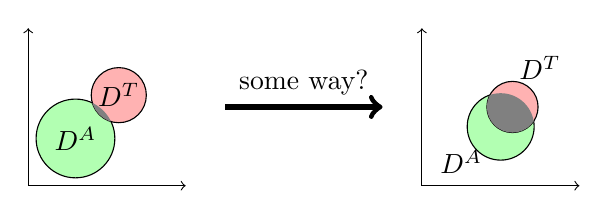
\begin{tikzpicture} [scale = 0.5]
		    \draw [->] (0,0) -- (4,0);
		    \draw [->] (0,0) -- (0,4);
		    
			\draw[fill=green!30] (1.2,1.2) circle (1) node {$D^A$};
			\draw[fill=red!30] (2.3,2.3) circle (0.7) node {$D^T$};

		    \begin{scope}
		    \clip (1.2,1.2) circle (1);
		    \fill [color = gray] (2.3,2.3) circle (0.7);
		    \end{scope}

		    \draw [->] (10,0) -- (14,0);
		    \draw [->] (10,0) -- (10,4);


		    \draw[fill=green!30] (12,1.5) circle (0.85);
			\draw[fill=red!30] (12.3,2) circle (0.65);		   

		    \begin{scope}
		    \clip (12,1.5) circle (0.85);
		    \fill [color = gray] (12.3,2) circle (0.65);
		    \end{scope}

		    \node () at (11,0.6) {$D^A$};
		    \node () at (13, 3) {$D^T$};

		    \draw[->, line width = 2pt] (5,2) -- (9,2) node[pos=0.5, above] {some way?};
		\end{tikzpicture}
		\end{center}

		\item Seek a special kernel function \alert{$\varphi(x)$} which minimizes the difference 
			\begin{itemize}
				\item Find the optimal weights \alert{($d_1, d_2, ..., d_M$)} of multiple kernels

		\begin{center}
		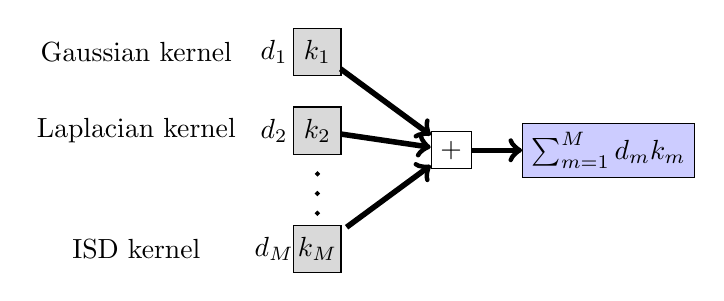
\begin{tikzpicture} [scale = 0.5]
		\draw[fill = gray!30] (0, 0) rectangle (1.2,1.2) node[pos = 0.5] (dm) {$k_M$};
		\node at (-0.5, 0.6) {$d_M$};
		\node at (-4, 0.6) {ISD kernel};


		\draw[fill=black] (0.6, 1.5) circle (0.05);
		\draw[fill=black] (0.6, 2) circle (0.05);
		\draw[fill=black] (0.6, 2.5) circle (0.05);

		\draw[fill = gray!30] (0, 3) rectangle (1.2,4.2) node[pos = 0.5] (d2) {$k_2$};
		\node at (-0.5, 3.6) {$d_2$};
		\node at (-4, 3.6) {Laplacian kernel};


		\draw[fill = gray!30] (0, 5) rectangle (1.2, 6.2) node[pos = 0.5] (d1) {$k_1$};
		\node at (-0.5, 5.6) {$d_1$};
		\node at (-4, 5.6) {Gaussian kernel};

		\node[draw] (plusOne) at (4, 3.1) {$+$};

		\node[draw, fill = blue!20] (sumOne) at (8, 3.1) {$\sum_{m=1}^{M} d_m k_m$};

		% edges
		\draw[->, line width = 2pt] (d1) -- (plusOne);
		\draw[->, line width = 2pt] (d2) -- (plusOne);
		\draw[->, line width = 2pt] (dm) -- (plusOne);
		\draw[->, line width = 2pt] (plusOne) -- (sumOne);


		\end{tikzpicture} 
		\end{center}


			\end{itemize}

	\end{itemize}
\end{frame}

\begin{frame}
	\begin{itemize}
		\item Define the mismatch between $D^A$ and $D^T$ as 
\begin{equation}
DIST_k(\mathcal{D}^A, \mathcal{D}^T) = \norm{\frac{1}{n_A} \sum_{i=1}^{n_A} \varphi(x_i^A) - \frac{1}{n_T} \sum_{i=1}^{n_T} \varphi (x_i^T)}
\end{equation}

		\item Simplify the square of equation (4) to
\begin{equation}
DIST_k^2(\mathcal{D}^A, \mathcal{D}^T) = \text{tr}(\mathbf{KS})
\end{equation}

where $\mathbf{s} = [\underbrace{\frac{1}{n_A}, ..., \frac{1}{n_A}}_\text{$n_A$}, \underbrace{\frac{-1}{n_T},...,\frac{-1}{n_T}}_\text{$n_T$}] ^T$, $\mathbf{S = s s^T }$, $\mathbf{K = \begin{bmatrix} K^{A,A} & K^{A,T} \\ K^{T, A} & K^{T,T}\\  \end{bmatrix}}$

	\item Incorporate \alert{$\mathbf{d} = [d_1, d_2, ..., d_M]^T$} into equation (5)
\begin{equation}
DIST_k^2(\mathcal{D}^A, \mathcal{D}^T) = \Omega(\mathbf{d}) = \mathbf{h^T d}
\end{equation}

where $\mathbf{h} = [tr(\mathbf{K_1 S}), \cdots, tr(\mathbf{K_MS})]^T$, and $\mathbf{K_m} = [\varphi(x)^T \varphi(x)]$ is the $m$th base kernel matrix 

	\end{itemize}
\end{frame}

\begin{frame}
	\begin{itemize}
		\item Optimization problem of DTSVM: 
			\begin{enumerate}
			    \item Distribution mismatch \tikz[na] \node[coordinate] (n1) {};
				\item SVM structural risk function \tikz[na] \node[coordinate] (n2) {};
			\end{enumerate}

			\begin{equation}
			\text{minimize} \quad G(\mathbf{d}) = 
			\tikz[baseline]{\node[fill=green!20,anchor=base] (t1)
			{$\frac{1}{2} \Omega^2(\mathbf{d})$};}
			+ \theta 
			\tikz[baseline]{\node[fill=red!20,anchor=base] (t2)
			{$J(\mathbf{d})$};}
			\end{equation} 

			where 
			\resizebox{.8 \textwidth}{!}{ 
			  $J(\mathbf{d}) = \underset{\boldsymbol{\alpha}}{\max} \; \sum_i \alpha_i - \frac{1}{2} \sum_{i,j} y_i y_j \alpha_i \alpha_j  (\sum_{m=1}^M d_m \; \varphi_m (x_i) ^T \varphi_m (x_j))$ 
			}


			\begin{tikzpicture}[overlay]
				\path[->, green, thick] (n1) edge [bend left] (t1); 
				\path[->, red!20, thick] (n2) edge [bend left] (t2); 
			\end{tikzpicture}

		\item Iteratively update coefficient $\mathbf{d}$ and the dual variable $\boldsymbol{\alpha}$

			\begin{enumerate}
				\item Update the dual variable $\boldsymbol{\alpha}$\\
				\item Update the coefficient $\mathbf{d}$ using \alert{gradient descent method} \\
				\begin{equation}
				\mathbf{d}_{t+1} = (1 - \eta_t) \mathbf{d}_{t} + \eta_t \mathbf{d}_t^{new}
				\end{equation}

				where 
				\resizebox{.76 \textwidth}{!}{ 		
				$\mathbf{d}_t^{new} = \theta(\mathbf{h h^T} + \varepsilon \mathbf{I_M})^{-1} \mathbf{q}$, 

				$\mathbf{q} = [\frac{1}{2}(\boldsymbol{\alpha}_t \diamond \mathbf{y})^T \mathbf{K}_1 (\boldsymbol{\alpha}_t \diamond \mathbf{y}), \cdots, \frac{1}{2}(\boldsymbol{\alpha}_t \diamond \mathbf{y})^T \mathbf{K}_M (\boldsymbol{\alpha}_t \diamond \mathbf{y})]$},

				$\eta_t$ is the learning rate.
			\end{enumerate}

		\item Final decision function
		\begin{equation}
		f(x) = \sum_{i=1}^{n} {\alpha}_i y_i \bigg(\sum_{m=1}^{M} d_m \mathbf{K}_m(x_i, x) \bigg) + b
		\end{equation}

	\end{itemize}
\end{frame}

\subsection{Adaptive MKL}
\begin{frame}{Adaptive Multiple Kernel Learning \cite{duan2012visual} (A-MKL)}
	\begin{itemize}

		\item Adaptive SVM
			\begin{equation}
			f(x) = 
			\tikz[baseline]{\node[fill=green!20,anchor=base] (t1)
			{$\sum_{k=1}^M t_k f_{k}^A(x)$};} 
			+ \Delta f(x)
			\end{equation}

		\item Domain Transfer SVM
			\begin{equation}
			f(x) = 
			\tikz[baseline]{\node[fill=red!20,anchor=base] (t2)
			{$\sum_{m=1}^{M} d_m w_m^T \varphi_m(x)$};} + b 
			\end{equation}

		\item Adaptive MKL
			\begin{equation}
			f(x) = 
			\tikz[baseline]{\node[fill=green!20,anchor=base] (n1)
			{$\sum_{p=1}^{P} \beta_p f_p(x)$};}
			+ 
			\tikz[baseline]{\node[fill=red!20,anchor=base] (n2)
			{$\sum_{m=1}^{M} d_m w_m^T \varphi_m(x)$};} + b 
			\end{equation}

		\begin{tikzpicture}[overlay]
			\path[->, green, thick] (t1) edge [bend right] (n1); 
			\path[->, red, thick] (t2) edge [bend left] (n2); 
		\end{tikzpicture}

			\begin{itemize}
				\item Seek a hyperplane which is close to that of all labeled samples
				\item Reduce the mismatch of different domains
			\end{itemize}

	\end{itemize}

\end{frame}

\subsection{Experiments}
\begin{frame}{Experiments of Domain Adaptation Approaches}

\begin{itemize}

	\item Data set
	
  \begin{table}[!ht]
    \begin{center}
      \scalebox{0.7}{
      \begin{tabular}{cccccccc}
      \hline
      \head{} & \head{Wedding} & \head{Sports} & \head{Show} & \head{Picnic} & \head{Parade} & \head{Birthday} & \head{Total}\\
      \hline
      Kodak & 27 & 75 & 57 & 6 & 14 & 16 & 195\\
      Youtube & 91 & 260 & 200 & 85 & 119 & 151 & 906\\
      \hline
      \end{tabular}
    }
    \end{center}
    \caption{Number of videos in each class from Kodak and Youtube}
  \end{table}

  \item Distances using various approaches

	\begin{table}[!ht]
	  \begin{center}
	  \scalebox{0.7}{
	    \begin{tabular} {cl}
	    \hline
	    \head{Setting Name} & \head{Content}\\
	    \hline
	    MAP(1) & Level 0 distance in Aligned Space-Time Pyramid Matching \\
	    MAP(2) & \alert{unaligned} Level 1 distance in Aligned Space-Time Pyramid Matching\\
	    MAP(3) & \alert{aligned} Level 1 distance in Aligned Space-Time Pyramid Matching \\

	    MAP(4) & Level 0 distance using histograms built in \alert{``tfc''} weighting scheme \\

	    MAP(5) & Level 0 distance using histograms built by \alert{straightforward soft assignment} \\
	    MAP(6) & Level 0 distance using histograms built by \alert{GMM soft assignment} \\

	    MAP(7) & \vtop{\hbox{\strut distances calculated by \alert{specialized GMMs} built on 128 dimensional SIFT} \hbox{\strut features with spherical covariance}} \\

	    MAP(8) & \alert{two} set of distances: MAP(3) + MAP(6) \\
	    \hline
	    \end{tabular}
	  }
	    \end{center}
	    \caption{Experimental distance set}
	\end{table}

\end{itemize}
\end{frame}

\begin{frame}
	\begin{itemize}
		\item Base kernel matrices
			\begin{columns}
				\column{0.33\textwidth}
					\begin{table}[!ht]
					    \begin{center}
					      \scalebox{0.75}{
					      \begin{tabular}{cc}
					      \hline
					      \head{Kernel type} & \head{Kernel function}\\
					      \hline
					      Gaussian & $\exp(-\gamma D^2(I_i, I_j)$ \\
					      Laplacian & $\exp(- \sqrt{\gamma} D(I_i, I_j)$ \\
					      ISD & $\frac{1}{\gamma D^2(I_i, I_j) + 1}$ \\
					      ID & $\frac{1}{\sqrt{\gamma}D(I_i, I_j) + 1}$\\
					      \hline
					      \end{tabular}
					      }
					    \end{center}
					\end{table}

				\column{0.67\textwidth}
					\begin{itemize}
						\item $D(I_i, I_j)$ represents the distance between $I_i$ and $I_j$

						\item $\gamma = 2^l \gamma_0$
							\begin{itemize}
								\item $\gamma_0 = \frac{1}{A}$, $A$ is the mean value of the squared distances between training samples

								\item $l \in \alert{(-3, -2,\cdots, 1)}$
							\end{itemize}
						
						\item \alert{$4 \times 5$} combinations $\rightarrow$ 20 base kernel matrices
					\end{itemize}
			\end{columns}

		\item Division of training and testing samples
			\begin{itemize}
				\item 3 videos for each class in Kodak domain as $\mathcal{D}_l^T$, and the left 

				\item the left Kodak videos as $\mathcal{D}_u^T$

				\item all Youtube videos as fully labeled $\mathcal{D}^A$ 
			\end{itemize}

		\item Evaluation metric: Mean Average Precision
			
			% \begin{equation}
			% \resizebox{.25\hsize}{!}{
			% $AP = \frac{1}{R} \sum_{j} \frac{R_j}{j} \times I_j$}
			% \end{equation} 

			% \begin{itemize}
			% 	\item $R_j$ be the number of true relevant videos in the top $j$ list

			% 	\item $I_j = 1$ if and only if the $j$th video is true relevant, otherwise $I_j = 0$ 
			% \end{itemize}
	\end{itemize}	
\end{frame}

\begin{frame}{Experimental Results}
	\begin{table}[!ht]
  \begin{center}
  \scalebox{0.7}{

    \begin{tabular} {ccccccc}
    \hline
    \head{} &\head{    \tikz[baseline]{\node[anchor=base] (one1) {SVM\textunderscore T};}              } &\head{SVM\textunderscore AT} &\head{FR} &\head{A-SVM}  &\head{DTSVM} &\head{A-MKL} \\
    \hline
    MAP(1) & $44.33 \pm 2.61$ & $52.21 \pm2.54$ & $52.33 \pm 2.20$ & $47.03 \pm3.26$ & $47.14 \pm3.26$ & $54.29 \pm 2.21$ \\

    MAP(2) & $43.55 \pm3.46$&  $55.37 \pm2.26$&  $55.95 \pm 3.79$  &$45.86 \pm4.39$  &$50.97 \pm 1.38$ & $54.26 \pm 3.46$ \\

    MAP(3) & $44.08 \pm 3.25$ & $57.56 \pm3.02$ & $53.91 \pm 1.48$ & $45.42 \pm 3.62$  & $53.32 \pm 2.56$ & $\mathbf{57.45 \pm 1.64}$ \\

    MAP(4) &
    $ 45.27 \pm 1.63$ & $ 51.83 \pm 2.27$ & $52.55 \pm 2.00$ & $45.94 \pm 1.70 $  & $52.31  \pm 2.56$ & $53.05\pm 2.21$ \\

    MAP(5) & 
    $44.79 \pm 2.55$ & $47.80 \pm 1.67$ & $51.89 \pm 1.99$ & $47.41 \pm 3.13$ & $45.05 \pm 4.07$ & $51.08 \pm 2.87$ \\

    \tikz[baseline]{\node[anchor=base] (two1) {MAP(6)};} & $45.20 \pm 3.04$ & $56.90 \pm 2.79$ & $54.03\pm 4.02$ & $46.62 \pm 3.14 $ & $53.41 \pm 3.29$ & \tikz[baseline]{\node[anchor=base] (two2) {$\mathbf{59.16 \pm 3.38}$};} \\

    MAP(7) &
    $32.91 \pm 2.20$ & $33.15 \pm 1.78$ & $41.78 \pm 3.98 $ &$37.07 \pm 3.52$& $\mathbf{46.61 \pm 2.41}$ & $35.88 \pm 1.98$ \\

    MAP(8) & $ 44.69\pm 2.84$ &   \tikz[baseline]{\node[anchor=base] (one2) {$ 60.21 \pm 1.94 $};} & $55.29 \pm 3.00$ & $46.28 \pm 4.23 $  & $ 57.01 \pm 2.45 $ & \alert{$\mathbf{61.40 \pm 1.91}$} \\

    \hline
    \end{tabular}
    }

    \end{center}
    \caption{Means and standard deviations (percent) of MAPs over six events}
\end{table}



		\begin{enumerate}
		 	\item  In all cases, \tikz[baseline, inner sep=0] \node[anchor=base] (one3) {SVM\_AT}; performed better than SVM\_T 
		 	\item \tikz[na] \node[coordinate] (two3) {two3};  Gaussian soft assignment outperformed the other approaches

		 	\item DTSVM performed amazingly in MAP(7)
		 	\item A-MKL performed the best by selecting two distance matrices smartly
		 	
		\end{enumerate}

		\begin{tikzpicture}[overlay]
			% first item
			 \draw[red!40,thick,line width = 2] ($(one1.north west)+(-1,-0.5)$)  rectangle ($(one2.south east)+(-2,0.5)$) ;
			 \draw [->, line width = 2, red!40] ($(one2.south east)+(-3,0.4)$) -- (one3);

			 % second item
			 \draw[green!40,thick,line width = 2] ($(two1.north west)+(-0.2,0.1)$)  rectangle ($(two2.south east)+(-1,0.35)$) ;
			 \path[green, line width = 2, green!40, ->] ($(two1.south west)+(-0.2,0.5)$) edge [out = -100, in = 180] (two3);

		\end{tikzpicture}

\end{frame}

\begin{frame} {Recognition Accuracy as Evaluation Metric}
	\begin{itemize}
		\item Recognition accuracy is defined as 
			\begin{equation}
			\text{recognition accuracy} = \frac{\text{correct predictions}}{\text{number of testing samples}}
			\end{equation}
		\item SVM multi-class classification


			\begin{columns}
				\column{0.4\textwidth}
					\begin{center}
					one-vs-all
					\end{center}
					\vspace{3 mm}
					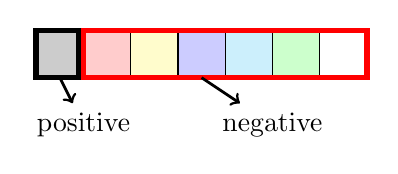
\begin{tikzpicture} [scale=0.3]

						\draw[fill=black!20] (0,0) rectangle (2, 2);
						\draw[fill=red!20] (2,0) rectangle (4, 2);
						\draw[fill=yellow!20] (4,0) rectangle (6, 2);
						\draw[fill=blue!20] (6,0) rectangle (8, 2);
						\draw[fill=cyan!20] (8,0) rectangle (10, 2);
						\draw[fill=green!20] (10,0) rectangle (12, 2);


						\draw[line width = 2pt, black] (0,0) rectangle (1.8, 2);
						\draw[line width = 2pt, red] (2,0) rectangle (14, 2);

						\coordinate (A1) at (1,0);
						\coordinate (B1) at (7,0);

						\node (A2) at (2, -2) {positive};
						\node (B2) at (10, -2) {negative};

						\draw[->, line width = 1pt] (A1) -- (A2);
						\draw[->, line width = 1pt] (B1) -- (B2);

					\end{tikzpicture}

					$n$ classes $\rightarrow$ $n$ classifiers 


				\column{0.4\textwidth}
					\begin{center}
					one-vs-one
					\end{center}

					\vspace{3 mm}
					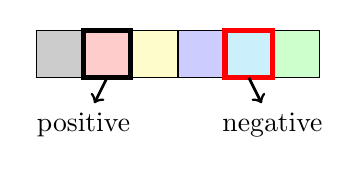
\begin{tikzpicture} [scale=0.3]

						\draw[fill=black!20] (0,0) rectangle (2, 2);
						\draw[fill=red!20] (2,0) rectangle (4, 2);
						\draw[fill=yellow!20] (4,0) rectangle (6, 2);
						\draw[fill=blue!20] (6,0) rectangle (8, 2);
						\draw[fill=cyan!20] (8,0) rectangle (10, 2);
						\draw[fill=green!20] (10,0) rectangle (12, 2);


						\draw[line width = 2pt, black] (2,0) rectangle (4, 2);
						\draw[line width = 2pt, red] (8,0) rectangle (10, 2);

						\coordinate (A1) at (3,0);
						\coordinate (B1) at (9,0);

						\node (A2) at (2, -2) {positive};
						\node (B2) at (10, -2) {negative};

						\draw[->, line width = 1pt] (A1) -- (A2);
						\draw[->, line width = 1pt] (B1) -- (B2);

					\end{tikzpicture}
					$n$ classes $\rightarrow$ $\frac{n(n-1)}{2}$ classifiers 
			\end{columns}

			




	\end{itemize}

\end{frame}

\begin{frame}
		\begin{table}[!ht]
	  	\centering
	  	\scalebox{0.6}{
	    \begin{tabular} {cccccccc}
	    \hline
	    \head{} &\head{SVM\textunderscore T} &\head{SVM\textunderscore AT} &\head{FR} &\head{A-SVM}  &\head{DTSVM} &\head{A-MKL} \\
	    \hline
	    one-vs-all & $49.94 \pm 6.96 $ & $ 57.85\pm 1.91$ & $57.18\pm8.59$ & $ 48.25\pm8.43$  & $ 55.82\pm0.83$ & $ \mathbf{58.87 \pm 0.90}$ \\
	    
	    one-vs-one & $ 33.67\pm 14.67$ & $ 51.64\pm 0.45 $ & $57.18 \pm 6.21$ & $36.05 \pm 12.62$ & $50.85\pm0.80$ & $ 55.14\pm 2.10$ \\
	    \hline
	    \end{tabular}
	    }

	    \caption{Means and standard deviations (percent) of average recognition accuracies}
		\end{table}

		\begin{table}[!ht]
			\centering
		  \scalebox{0.6}{
		    \begin{tabular} {cccccccc}
		    \hline
		    \head{} &\head{SVM\textunderscore T} &\head{SVM\textunderscore AT} &\head{FR} &\head{A-SVM} &\head{DTSVM} &\head{A-MKL} \\
		    \hline
		    one-vs-all & $0.98$ & $8.54$ & $10.53$ & $12.52$ & $11.33$ & $27.87$ \\
		    
		    one-vs-one & $1.49$ & $4.08$ & $5.68$ & $7.16$ & $5.05$ & $10.94$\\
		    \hline
		    \end{tabular}
		    }

		    \caption{Average running time (seconds)}
		\end{table}

		\begin{columns}
			\column{0.5\textwidth}
					\begin{figure}[!ht]
						\centering
						  \includegraphics[scale = 0.25]{./onevsone.png}
						\end{figure}

			\column{0.7\textwidth}
				\begin{itemize}
					\item \scriptsize{One-vs-all outperformed one-vs-one}
					\item \scriptsize{Trade-offs between running time and accuracy}
						\begin{enumerate}
							\item \scriptsize{One-vs-all requires more time}
							\item \scriptsize{Domain adaptations require more time}
						\end{enumerate}
				\end{itemize}
		\end{columns}

\end{frame}
\section{Conclusion}
\begin{frame}{Conclusion}

	\begin{itemize}
		\item What have been done in this FYP
			\begin{enumerate}
				\item Successfully implemented a recognition system to recognize videos
				\item Explored 4 various approaches to recognize videos
				\item Studied and implemented 4 domain adaptation methods to boost the performance
				\item Designed and developed a web application to demonstrate the work
			\end{enumerate}

		\item Future recommendations
			\begin{enumerate}
				\item Incorporate more types of features: space-time feature and acoustic feature
				\item Employ more attribute detectors 
				\item Combine various domain adaptation methods
			\end{enumerate}
	\end{itemize}
\end{frame}

\section{Demo}
\begin{frame}
	\begin{center}
	\Huge{Demo}
	\end{center}
\end{frame}

\section{References}
\bibliographystyle{IEEEtranS}
\bibliography{reference}
\end{document}